% Softwaredesign af PSoC på PSoC
\subsection{PSoC (PSoC)} \label{sec:sw_design_psoc_psoc}

PSoC'en blev sat ind relativt sent i implementeringsfasen. Hvilket har betydet at designfasen påbegyndte ret sent.
PSoC'ens formål, hardware- såvel som softwaremæssigt, er at simplificere \IIC kommunikation ved at interagere som en multi-master-slave enhed, som kan kommunikere som \IIC slave og samtidig som \IIC master overfor distancesensorerne. 
Raspbery Pi er udelukkende i stand til at være master, hvilket fjerner meget funktionalitet fra hvad formålet med sensorerne er. 
PSoC'en aflaster processoren på Pi'en, da \IIC kommunikationen, som er meget højt prioriteret, ville Pi'en konstant være forstyrret i relativt store tidsintervaller når der sendes og modtages data. 
Ved at implementere sensorene på PSoC'en kan disse også for den anbefalede på 100ms tid til at foretage deres læse/skrive cyklus. 
I første omgang var det meningen at PSoC'en skulle læses hver gang der var brug for noget specifikt data fra en individuel sensor eller fra tachometeret. 
Dette viste sig dog uhensigtsmæssigt, da PSoC'en da ville blive læst fem gange hurtigt efter hinanden, og dette ville forhindre sensorerne i at færdiggøre deres rutine. Derfor blev der sidenhen implementeret et andet program på Pi'en. 

\begin{figure}[h]
\centering
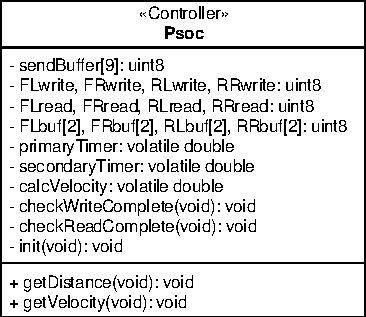
\includegraphics[]{../fig/diagrammer/psoc/cd_psoc.pdf}
\caption{Klassebeskrivelse for main på PSoC'en}
\label{fig:cd_main_psoc}
\end{figure}

\clearpage

\textbf{Attributter}

\begin{table}[h]
	\begin{tabularx}{\textwidth}{| L{3cm} | Z | L{10cm} |} \hline
	Navn 
	& Type 
	& Beskrivelse \\\hline
	
	\texttt{sendBuffer[9]}												 
		& \texttt{uint8}	
		& Array af typen int til indhold af aflæst sensordata, der skal læses af PI'en.\\\hline
	
	\texttt{FLwrite \newline FRwrite\newline RLwrite\newline RRwrite}	 
		& \texttt{uint8} 	
		& Variabel af typen const uint8 indeholdende write kommando til hhv. Front Left, Right og Rear Left, Right distance sensor.\\\hline
	
	\texttt{FLread\newline FRread\newline RLread\newline RRread}		 
		& \texttt{uint8}	
		& Variabel af typen const uint8 indeholdende read kommando til hhv. Front Left, Right og Rear Left, Right distance sensor.\\\hline
	
	\texttt{FLbuf[2]\newline FRbuf[2]\newline RLbuf[2]\newline RRbuf[2]} 
		& \texttt{uint8}	
		& Variabel af typen uint8. Fungerer som read buffer for hhv. Front Left, Right og Rear Left, Right distance sensor.\\\hline
	
	\texttt{primaryTimer}												 
		& \texttt{double}	
		& Variabel af typen double som indeholder en aflæst timerværdi.\\\hline
	
	\texttt{secondaryTimer}												 
		& \texttt{double}	
		& Variabel af typen double som indeholder den tidligste aflæste timerværdi fra primaryTimer.\\\hline
	
	\texttt{calcVelocity}												 
		& \texttt{volatile double}		
		& Variabel af typen double som indeholder den udregnede værdi i km/t gange 10.\\\hline
	
	\end{tabularx}
	\caption{Attributter for main på PSoC'en}
	\label{table:attr_psoc_main}
\end{table}

\clearpage

\textbf{Metoder}

\begin{table}[h]
	\begin{tabularx}{\textwidth}{| L{2.5 cm} | Z |} \hline
	Prototype 	& \texttt{void init(void)} 			\\\hline
	Parametre 	& \texttt{void} 					\newline \\\hline
	Returværdi	& \texttt{void} 					\newline \\\hline
	Beskrivelse	& Initierer alle dele af PSoC'en. 	\newline \\\hline
	\end{tabularx}
	\caption{Metodebeskrivelse for \texttt{init()} i PSoC main}
	\label{table:psoc_init}
\end{table}

\begin{table}[h]
	\begin{tabularx}{\textwidth}{| L{2.5 cm} | Z |} \hline
	Prototype 	& \texttt{void checkWriteComplete(void)}\\\hline
	Parametre 	& \texttt{void}  						\newline \\\hline
	Returværdi	& \texttt{void} 						\newline \\\hline
	Beskrivelse	& Ventetid mellem hver write til distance sensorer. \newline \\\hline
	\end{tabularx}
	\caption{Metodebeskrivelse for \texttt{checkWriteComplete} i PSoC main}
	\label{table:psoc_writecomplete}
\end{table}

\begin{table}[h]
	\begin{tabularx}{\textwidth}{| L{2.5 cm} | Z |} \hline
	Prototype 	& \texttt{void checkReadComplete(void)} \\\hline
	Parametre 	& \texttt{void}  						\newline \\\hline
	Returværdi	& \texttt{void} 						\newline \\\hline
	Beskrivelse	& Ventetid mellem hver read til distance sensorer. \newline \\\hline	
	\end{tabularx}
	\caption{Metodebeskrivelse for \texttt{checkReadComplete} i PSoC main}
	\label{table:psoc_readcomplete}
\end{table}

\begin{table}[h]
	\begin{tabularx}{\textwidth}{| L{2.5 cm} | Z |} \hline
	Prototype 	& \texttt{void getDistance(void)} 	\\\hline
	Parametre 	& \texttt{void} 					\newline \\\hline
	Returværdi	& \texttt{void} 					\newline \\\hline
	Beskrivelse	& Kommunikerer via \IIC til distance sensorerne hver især.  \\\hline
	\end{tabularx}
	\caption{Metodebeskrivelse for \texttt{getDistance()} i PSoC main}
	\label{table:psoc_getdistance}
\end{table}

\clearpage

\begin{table}[h]
	\begin{tabularx}{\textwidth}{| L{2.5 cm} | Z |} \hline
	Prototype 	& \texttt{void getVelocity(void)} 	\\\hline
	Parametre 	& \texttt{void}						\newline \\\hline
	Returværdi	& \texttt{void} 					\newline \\\hline
	Beskrivelse	& Funktionen fejltjekker værdien udregnet i my\_ISR, og gemmer den i sendBufferen. \newline \\\hline
	\end{tabularx}
	\caption{Metodebeskrivelse for \texttt{getVelocity()}}
	\label{table:psoc_getvelocity}
\end{table}

\begin{table}[h]
	\begin{tabularx}{\textwidth}{| L{2.5 cm} | Z |} \hline
	Prototype 	& \texttt{CY\_ISR(my\_ISR)} 		\\\hline
	Parametre 	& \texttt{void}						\newline \\\hline
	Beskrivelse	& Fungerer som interrupt service routine for PSoC'en, hver gang en magnet bliver detekteret af tachometeret.\newline \\\hline
	\end{tabularx}
	\caption{Metodebeskrivelse for \texttt{CY\_ISR(my\_ISR)}}
	\label{table:psoc_my_isr}
\end{table}

PSoC'ens program fungerer i store træk som vist på figur \ref{fig:sd_main_psoc}. Sekvensdiagrammet skal forstås som en forklaring af funktionalitet, som på højere abstraktionsniveau end selve koden giver en forståelse af hvad der sker inde i PSoC'en. 

\begin{figure}[h]
	\centering
	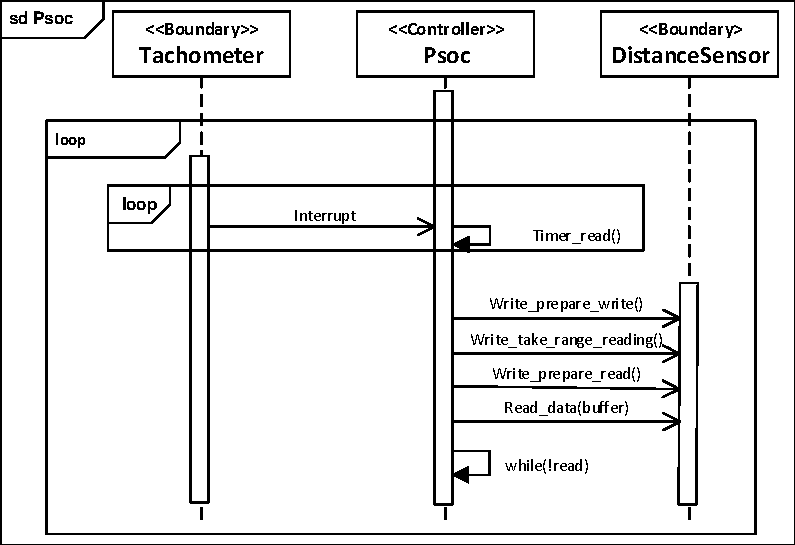
\includegraphics[]{../fig/diagrammer/psoc/sd_psoc.pdf}
	\caption{Sekvensdiagram af PSoC'ens funktionalitet}
	\label{fig:sd_main_psoc}
\end{figure}

\clearpage